%compiled with lualatex 15 Jan 2014, version: 4.40
\documentclass{scrreprt}

\usepackage[ngerman]{babel}
\usepackage{fontspec}
\usepackage{microtype,multicol,graphicx}
\usepackage{scrpage2}
\usepackage[textheight=27cm]{geometry}
\usepackage{wrapfig}
\usepackage{booktabs}
%\usepackage{picins}

\pagestyle{scrheadings}
\clearscrplain
\setmainfont[Ligatures=Common]{Linux Libertine O}
\setsansfont{Linux Libertine O}
\renewcommand{\thesection}{\Roman{section}}
\renewcommand*{\raggedsection}{\centering}

\begin{document}
%\vspace{-6cm}
\chapter*{Robotikpraktikum: Persistence of Vision}
\vspace{-.25cm}

\begin{center}
SS 2015\\
Betreuer: Gero Plettenberg\\
Supervisor: Thomas Kloepfer
\end{center}
\vspace{-.2cm}


\section{Projektziele}

%\vspace{-.25cm}
Ziel dieses Robotik-Projektes ist es, einen POV-Globus zu konzipieren, der beliebige Bilder anhand schnell rotierender LED's abbilden soll.\\
Unter Persistence of Vision (POV) versteht man allgemein die Trägheit des menschlichen Auges. Diese Eigenschaft kann bekanntlich genutzt werden, um durch sich schnell ändernde Bilder oder Lichtpulse einen ablaufenden Film zu erzeugen (ab ca. 24 Bilder/s).\\
Unser Projekt beinhaltet daher konkret die Planung und den Bau eines Globus, der von Nord- zu Südpol mit mehreren einzeln ansteuerbaren (RGB-) LED's ausgestattet ist. Durch Rotation des Globus und gezieltes, schnelles An- und Abschalten der Lichtquellen kann dabei -wie bei einem Bildschirm- jeder Punkt auf der sich rotierenden Kugel einzeln zum Leuchten gebracht werden. Hierzu wird ein Mini-Computer (z.B. Raspberry Pi) auf dem sich drehenden Globus angebracht, der die Aktivierung der RGB's und die Rotationsgeschwindigkeit genau aufeinander abstimmt.\\
In einem zweiten Schritt soll ein Interface zur interaktiven Steuerung des zu darstellenden Bildes erarbeitet werden.\\


\begin{center}
%\vspace{-.75cm}
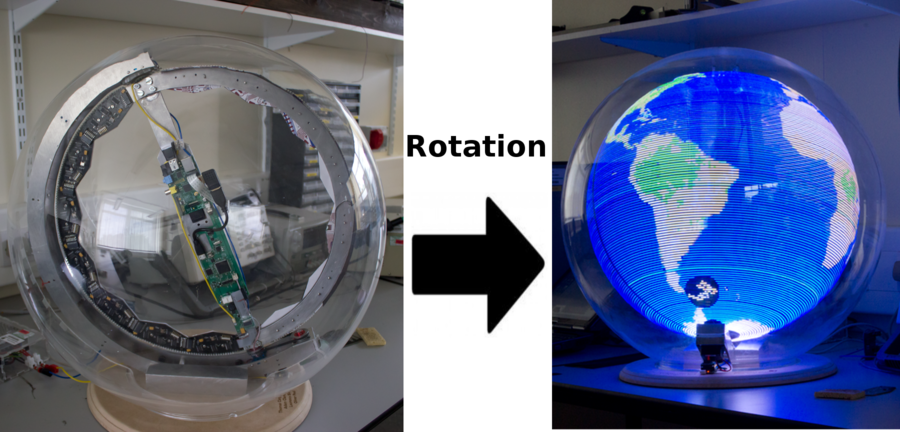
\includegraphics[height=.24\textwidth]{pov.png}\qquad\qquad
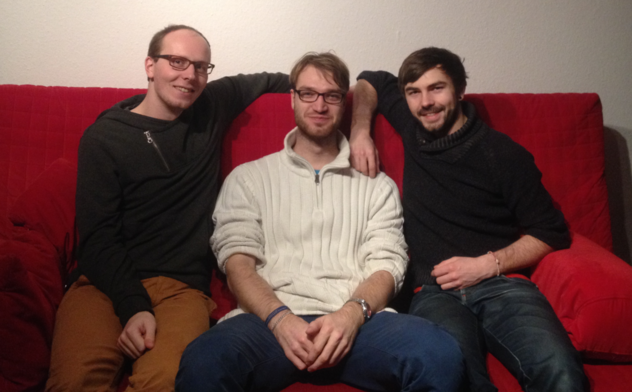
\includegraphics[height=.24\textwidth]{team.png}
\end{center}
%\vspace{-1cm}


\section{Milestones}

\begin{tabular}{ll}
\it{bis Mitte Juni:}&
\bullet\ genaues Konzept erarbeiten \& Materialien wählen (tech. Details\\
\vspace{.2cm}
&\ \ \ klären; Styroporkugel vs. Alu-Ring; Motor- und LED-Wahl etc.)\\
\vspace{.2cm}

\it{bis Ende Juni:}&
\bullet\ Ersten Aufbau realisieren \& Rotations-Timing justieren \\
\vspace{.2cm}

\it{bis Ende Juli:}&
\bullet\ Aufbau vervollständigen (LED's, Hülle etc) \& testen\\
\vspace{.2cm}

\it{bis Ende August:}&
\bullet\ Fine-Tuning der Mechanik\\
\vspace{.2cm}

\it{bis Mitte September:}&
\bullet\ Software-Steuerung vervollständigen: Interface erstellen\\
\vspace{.2cm}

\it{bis Ende September:}&
\bullet\ Poster \& Präsentation erstellen und Projekt vorstellen
\end{tabular}
%\vspace{-.25cm}




\section{Gruppenmitglieder}
%\vspace{-.25cm}
\begin{multicols}{3}
\begin{center}
Maximilian Hartmann\\
Master Physik 4. Semester\\
maximilian.hartmann@stud.uni-heidelberg.de\\
Tobias Buck\\
Master Physik 4. Semester\\
Buck@stud.uni-heidelberg.de\\
\ \\
Philipp Gernandt\\
Master Physik 2. Semester\\
Gernandt@stud.uni-heidelberg.de
\end{center}
\end{multicols}


\end{document}

